\documentclass{standalone}
\usepackage{tikz}
\usetikzlibrary{patterns, positioning}

\begin{document}
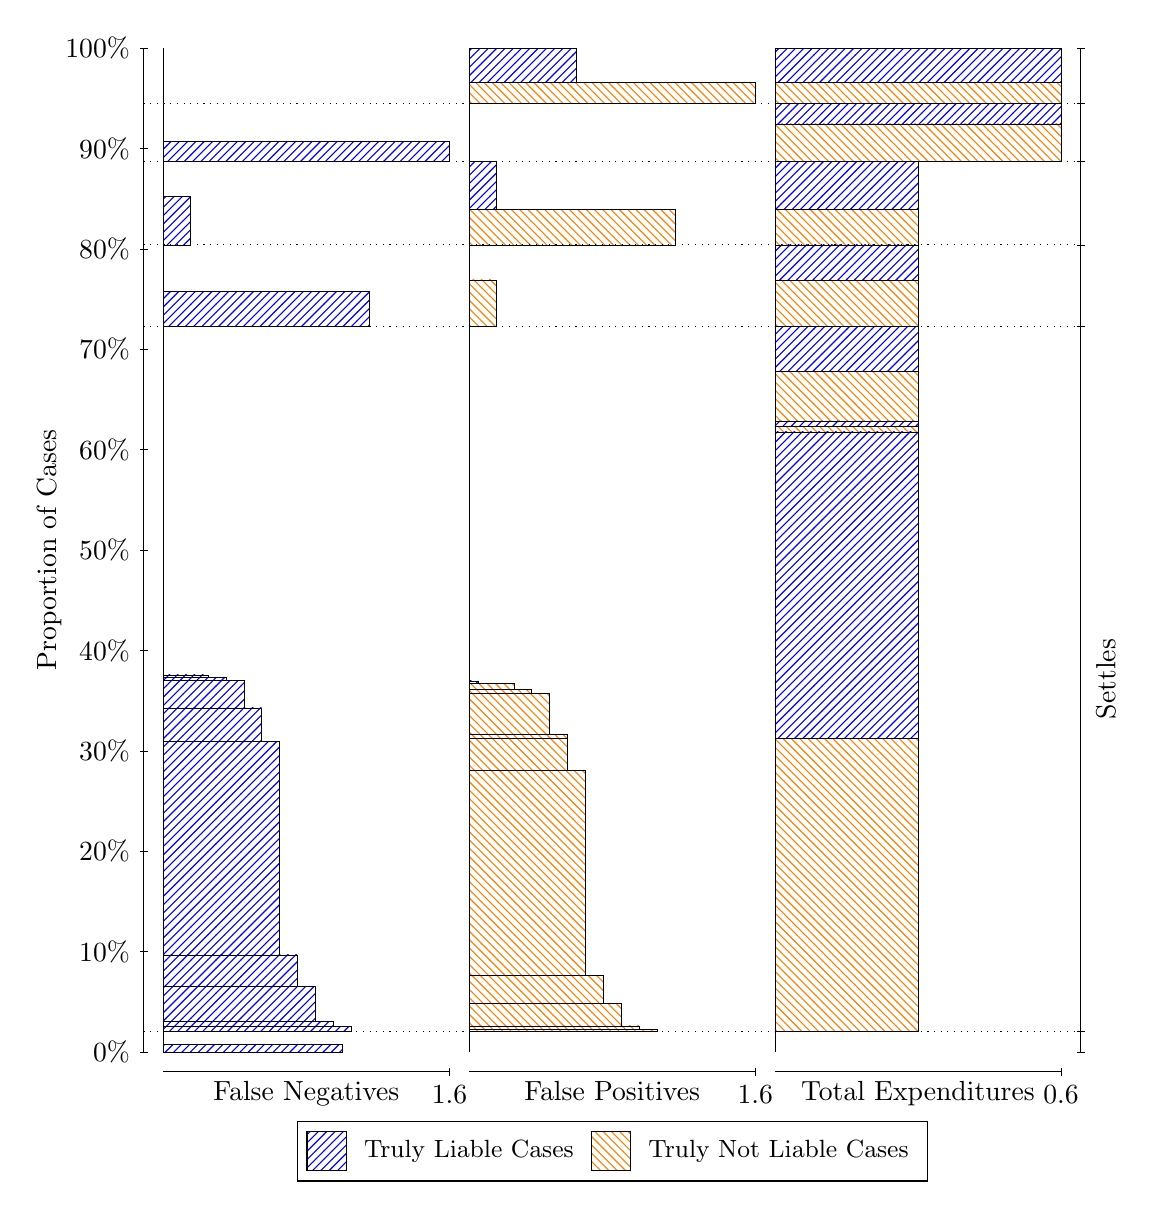
\begin{tikzpicture}
\draw[black, very thin] (1.5,1.75) -- (1.5,14.5);
\node[rotate=90, anchor=center] at (0.3, 8.125) {Proportion of Cases};
\draw[black, very thin] (1.45,1.75) -- (1.55,1.75);
\node[anchor=east] at (1.45, 1.75) {0\%};
\draw[black, very thin] (1.45,3.025) -- (1.55,3.025);
\node[anchor=east] at (1.45, 3.025) {10\%};
\draw[black, very thin] (1.45,4.3) -- (1.55,4.3);
\node[anchor=east] at (1.45, 4.3) {20\%};
\draw[black, very thin] (1.45,5.575) -- (1.55,5.575);
\node[anchor=east] at (1.45, 5.575) {30\%};
\draw[black, very thin] (1.45,6.85) -- (1.55,6.85);
\node[anchor=east] at (1.45, 6.85) {40\%};
\draw[black, very thin] (1.45,8.125) -- (1.55,8.125);
\node[anchor=east] at (1.45, 8.125) {50\%};
\draw[black, very thin] (1.45,9.4) -- (1.55,9.4);
\node[anchor=east] at (1.45, 9.4) {60\%};
\draw[black, very thin] (1.45,10.675) -- (1.55,10.675);
\node[anchor=east] at (1.45, 10.675) {70\%};
\draw[black, very thin] (1.45,11.95) -- (1.55,11.95);
\node[anchor=east] at (1.45, 11.95) {80\%};
\draw[black, very thin] (1.45,13.225) -- (1.55,13.225);
\node[anchor=east] at (1.45, 13.225) {90\%};
\draw[black, very thin] (1.45,14.5) -- (1.55,14.5);
\node[anchor=east] at (1.45, 14.5) {100\%};

\draw[black, very thin] (13.4,1.75) -- (13.4,14.5);
\draw[black, very thin] (13.35,1.75) -- (13.45,1.75);
\node[anchor=west] at (13.35, 1.75) {};
\draw[black, very thin] (13.35,2.0108) -- (13.45,2.0108);
\node[anchor=west] at (13.35, 2.0108) {};
\draw[black, very thin] (13.35,10.962) -- (13.45,10.962);
\node[anchor=west] at (13.35, 10.962) {};
\draw[black, very thin] (13.35,12) -- (13.45,12);
\node[anchor=west] at (13.35, 12) {};
\draw[black, very thin] (13.35,13.063) -- (13.45,13.063);
\node[anchor=west] at (13.35, 13.063) {};
\draw[black, very thin] (13.35,13.793) -- (13.45,13.793);
\node[anchor=west] at (13.35, 13.793) {};
\draw[black, very thin] (13.35,14.5) -- (13.45,14.5);
\node[anchor=west] at (13.35, 14.5) {};

\draw[black, very thin, pattern color=blue, pattern=north east lines] (1.75,1.75) rectangle (4.0208,1.8454);
\draw[black, very thin, pattern color=orange, pattern=north west lines] (1.75,1.8454) rectangle (1.75,2.0108);
\draw[black, very thin, pattern color=blue, pattern=north east lines] (1.75,2.0108) rectangle (4.1344,2.0772);
\draw[black, very thin, pattern color=blue, pattern=north east lines] (1.75,2.0772) rectangle (3.9073,2.1346);
\draw[black, very thin, pattern color=blue, pattern=north east lines] (1.75,2.1346) rectangle (3.6802,2.5834);
\draw[black, very thin, pattern color=blue, pattern=north east lines] (1.75,2.5834) rectangle (3.4531,2.9826);
\draw[black, very thin, pattern color=blue, pattern=north east lines] (1.75,2.9826) rectangle (3.226,5.6949);
\draw[black, very thin, pattern color=blue, pattern=north east lines] (1.75,5.6949) rectangle (2.999,6.1202);
\draw[black, very thin, pattern color=blue, pattern=north east lines] (1.75,6.1202) rectangle (2.7719,6.4686);
\draw[black, very thin, pattern color=blue, pattern=north east lines] (1.75,6.4686) rectangle (2.5448,6.5107);
\draw[black, very thin, pattern color=blue, pattern=north east lines] (1.75,6.5107) rectangle (2.3177,6.5399);
\draw[black, very thin, pattern color=orange, pattern=north west lines] (1.75,6.5399) rectangle (1.75,10.962);
\draw[black, very thin, pattern color=blue, pattern=north east lines] (1.75,10.962) rectangle (4.3615,11.406);
\draw[black, very thin, pattern color=orange, pattern=north west lines] (1.75,11.406) rectangle (1.75,12);
\draw[black, very thin, pattern color=blue, pattern=north east lines] (1.75,12) rectangle (2.0906,12.611);
\draw[black, very thin, pattern color=orange, pattern=north west lines] (1.75,12.611) rectangle (1.75,13.063);
\draw[black, very thin, pattern color=blue, pattern=north east lines] (1.75,13.063) rectangle (5.3833,13.318);
\draw[black, very thin, pattern color=orange, pattern=north west lines] (1.75,13.318) rectangle (1.75,13.793);
\draw[black, very thin, pattern color=orange, pattern=north west lines] (1.75,13.793) rectangle (1.75,14.059);
\draw[black, very thin, pattern color=blue, pattern=north east lines] (1.75,14.059) rectangle (1.75,14.5);
\draw[black, very thin, pattern color=orange, pattern=north west lines] (5.6333,1.75) rectangle (5.6333,1.9154);
\draw[black, very thin, pattern color=blue, pattern=north east lines] (5.6333,1.9154) rectangle (5.6333,2.0108);
\draw[black, very thin, pattern color=orange, pattern=north west lines] (5.6333,2.0108) rectangle (8.0177,2.0416);
\draw[black, very thin, pattern color=orange, pattern=north west lines] (5.6333,2.0416) rectangle (7.7906,2.0808);
\draw[black, very thin, pattern color=orange, pattern=north west lines] (5.6333,2.0808) rectangle (7.5635,2.3695);
\draw[black, very thin, pattern color=orange, pattern=north west lines] (5.6333,2.3695) rectangle (7.3365,2.7218);
\draw[black, very thin, pattern color=orange, pattern=north west lines] (5.6333,2.7218) rectangle (7.1094,5.3294);
\draw[black, very thin, pattern color=orange, pattern=north west lines] (5.6333,5.3294) rectangle (6.8823,5.7284);
\draw[black, very thin, pattern color=orange, pattern=north west lines] (5.6333,5.7284) rectangle (6.8823,5.7862);
\draw[black, very thin, pattern color=orange, pattern=north west lines] (5.6333,5.7862) rectangle (6.6552,6.3005);
\draw[black, very thin, pattern color=orange, pattern=north west lines] (5.6333,6.3005) rectangle (6.4281,6.3594);
\draw[black, very thin, pattern color=orange, pattern=north west lines] (5.6333,6.3594) rectangle (6.201,6.4329);
\draw[black, very thin, pattern color=blue, pattern=north east lines] (5.6333,6.4329) rectangle (5.7469,6.4622);
\draw[black, very thin, pattern color=blue, pattern=north east lines] (5.6333,6.4622) rectangle (5.6333,10.962);
\draw[black, very thin, pattern color=orange, pattern=north west lines] (5.6333,10.962) rectangle (5.974,11.556);
\draw[black, very thin, pattern color=blue, pattern=north east lines] (5.6333,11.556) rectangle (5.6333,12);
\draw[black, very thin, pattern color=orange, pattern=north west lines] (5.6333,12) rectangle (8.2448,12.452);
\draw[black, very thin, pattern color=blue, pattern=north east lines] (5.6333,12.452) rectangle (5.974,13.063);
\draw[black, very thin, pattern color=orange, pattern=north west lines] (5.6333,13.063) rectangle (5.6333,13.538);
\draw[black, very thin, pattern color=blue, pattern=north east lines] (5.6333,13.538) rectangle (5.6333,13.793);
\draw[black, very thin, pattern color=orange, pattern=north west lines] (5.6333,13.793) rectangle (9.2667,14.059);
\draw[black, very thin, pattern color=blue, pattern=north east lines] (5.6333,14.059) rectangle (6.9958,14.5);
\draw[black, very thin, pattern color=orange, pattern=north west lines] (9.5167,1.75) rectangle (9.5167,1.9154);
\draw[black, very thin, pattern color=blue, pattern=north east lines] (9.5167,1.9154) rectangle (9.5167,2.0108);
\draw[black, very thin, pattern color=orange, pattern=north west lines] (9.5167,2.0108) rectangle (11.333,5.7284);
\draw[black, very thin, pattern color=blue, pattern=north east lines] (9.5167,5.7284) rectangle (11.333,9.6261);
\draw[black, very thin, pattern color=orange, pattern=north west lines] (9.5167,9.6261) rectangle (11.333,9.6996);
\draw[black, very thin, pattern color=blue, pattern=north east lines] (9.5167,9.6996) rectangle (11.333,9.766);
\draw[black, very thin, pattern color=orange, pattern=north west lines] (9.5167,9.766) rectangle (11.333,10.397);
\draw[black, very thin, pattern color=blue, pattern=north east lines] (9.5167,10.397) rectangle (11.333,10.962);
\draw[black, very thin, pattern color=orange, pattern=north west lines] (9.5167,10.962) rectangle (11.333,11.556);
\draw[black, very thin, pattern color=blue, pattern=north east lines] (9.5167,11.556) rectangle (11.333,12);
\draw[black, very thin, pattern color=orange, pattern=north west lines] (9.5167,12) rectangle (11.333,12.452);
\draw[black, very thin, pattern color=blue, pattern=north east lines] (9.5167,12.452) rectangle (11.333,13.063);
\draw[black, very thin, pattern color=orange, pattern=north west lines] (9.5167,13.063) rectangle (13.15,13.538);
\draw[black, very thin, pattern color=blue, pattern=north east lines] (9.5167,13.538) rectangle (13.15,13.793);
\draw[black, very thin, pattern color=orange, pattern=north west lines] (9.5167,13.793) rectangle (13.15,14.059);
\draw[black, very thin, pattern color=blue, pattern=north east lines] (9.5167,14.059) rectangle (13.15,14.5);
\draw[black, dotted] (1.5,2.0108) -- (13.4,2.0108);
\draw[black, dotted] (1.5,10.962) -- (13.4,10.962);
\draw[black, dotted] (1.5,12) -- (13.4,12);
\draw[black, dotted] (1.5,13.063) -- (13.4,13.063);
\draw[black, dotted] (1.5,13.793) -- (13.4,13.793);
\draw[black, very thin] (1.75,1.5) -- (5.3833,1.5);
\node[anchor=north] at (3.5667, 1.5) {False Negatives};
\draw[black, very thin] (5.3833,1.45) -- (5.3833,1.55);
\node[anchor=north] at (5.3833, 1.45) {1.6};

\draw[black, very thin] (5.6333,1.5) -- (9.2667,1.5);
\node[anchor=north] at (7.45, 1.5) {False Positives};
\draw[black, very thin] (9.2667,1.45) -- (9.2667,1.55);
\node[anchor=north] at (9.2667, 1.45) {1.6};

\draw[black, very thin] (9.5167,1.5) -- (13.15,1.5);
\node[anchor=north] at (11.333, 1.5) {Total Expenditures};
\draw[black, very thin] (13.15,1.45) -- (13.15,1.55);
\node[anchor=north] at (13.15, 1.45) {0.6};


\node[black, centered, rotate=90] at (13.72, 6.4864) {Settles};





\draw (7.449999999999999,1.5) node[draw=none] (baseCoordinate) {};
\begin{scope}[align=center]
        \matrix[scale=0.5, draw=black, below=0.5cm of baseCoordinate, nodes={draw}, column sep=0.1cm]{
            \node[rectangle, draw, minimum width=0.5cm, minimum height=0.5cm, pattern=north east lines, pattern color=blue] {}; &
            \node[draw=none, font=\small] (B) {Truly Liable Cases}; &
            \node[rectangle, draw, minimum width=0.5cm, minimum height=0.5cm, pattern=north west lines, pattern color=orange] {}; &
            \node[draw=none, font=\small] (B) {Truly Not Liable Cases}; \\
            };
\end{scope}

\end{tikzpicture}
\end{document}